\documentclass{article}
\usepackage[letterpaper,margin=1in]{geometry}
\usepackage{xcolor}
\usepackage{fancyhdr}
\usepackage{amsmath}
\usepackage{graphicx}
\usepackage{float}

\pagestyle{fancy}

\lhead{\textit{\yourname}}
\rhead{\textit{PHYS 142}}
\thispagestyle{empty}

\setlength{\parindent}{0cm}
\setlength{\itemindent}{0cm}

\newcommand{\mytitle}{PHYS 142: Assignment 2}
\newcommand{\yourname}{Jessica Birky}

\begin{document}
\hrule \vspace{1pt} \hrule 
\begin{center}\Large \textbf{\sc \mytitle} \\
\normalsize \sc Jessica Birky (A13002163)
\end{center}
\hrule \vspace{1pt} \hrule 


\bigskip
\textbf{Question 1}: Design an experiment to simulate the tunneling time in a double potential well. \\

For the potential I use the parameterization 
\[V(x) = \alpha (x^2 - x_{min}^2)^2 \]
where I choose $\alpha = .02$ and $x_{min}=2.5$. \\ 

The initial condition is chosen to be the difference in the lowest two stationary stationary states for this potential:
\[|\psi_o\rangle = \frac{1}{\sqrt{2}} (|\phi_o\rangle - |\phi_1\rangle) \]
where $|\phi_o\rangle$ is the ground state and $|\phi_1\rangle$ is the first excited state. For simplification I use a gaussian approximation for the initial condition, choosing $\gamma = 1$ and the center to be at the the minimum of the potential well, $x_{min}$:
\[\psi_o(x) = e^{-\frac{\gamma}{2} (x-x_{min})^2} \]

Plot of the normalized initial condition and double potential well:
\begin{figure}[H]
\begin{center}
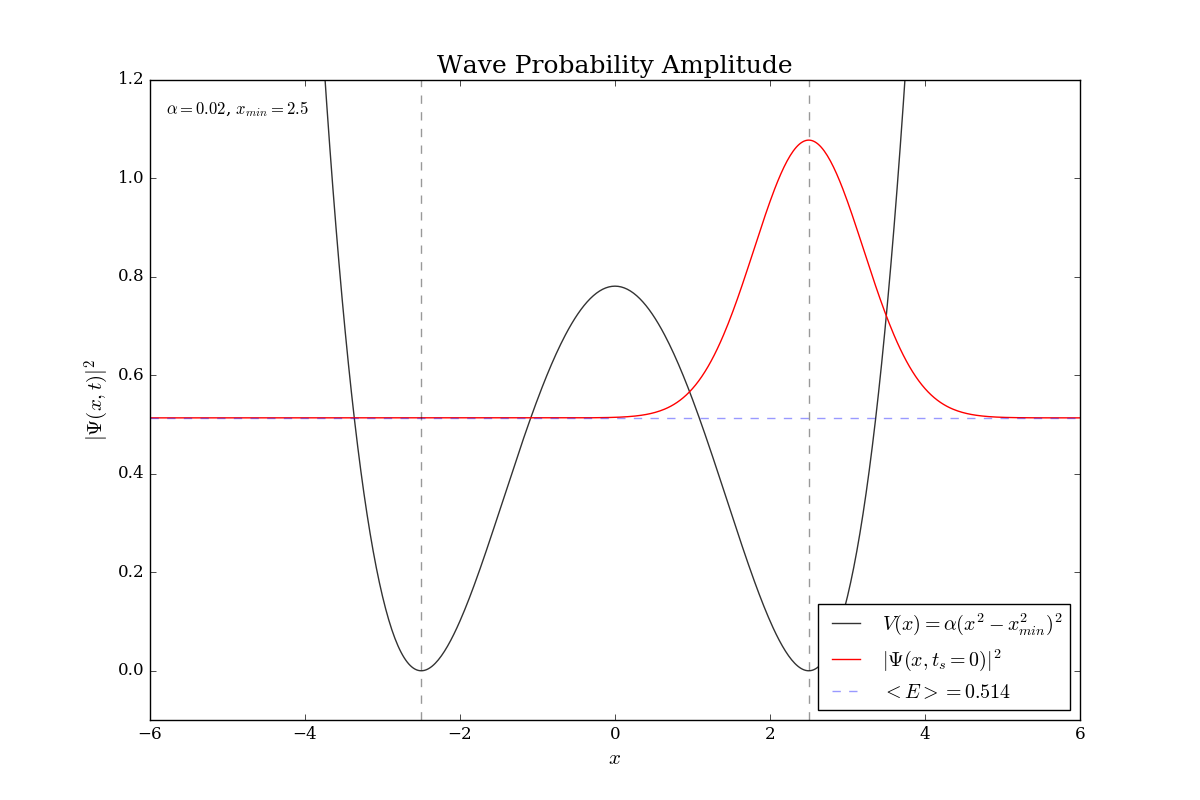
\includegraphics[width=16cm]{plots/phi_sq0.png} 
\end{center}
\end{figure}

The tunneling time for this experiment can be numerically estimated as the time it takes the expected position to go from $x_{min}$ to $-x_{min}$.


\bigskip
\textbf{Question 2}: Demonstrate how the wave function tunnels through the barrier with time. \\

\textit{Solution:} Evolution of the wave function was taken over 256 time steps, with classical period of oscillation $T_o=2\pi$, propagator caluclations in $T=\frac{T_o}{16}$ intervals, and N=8 time slices in each ($\Delta t=\frac{T_o}{128}$).
\begin{figure}[H]
\begin{center}
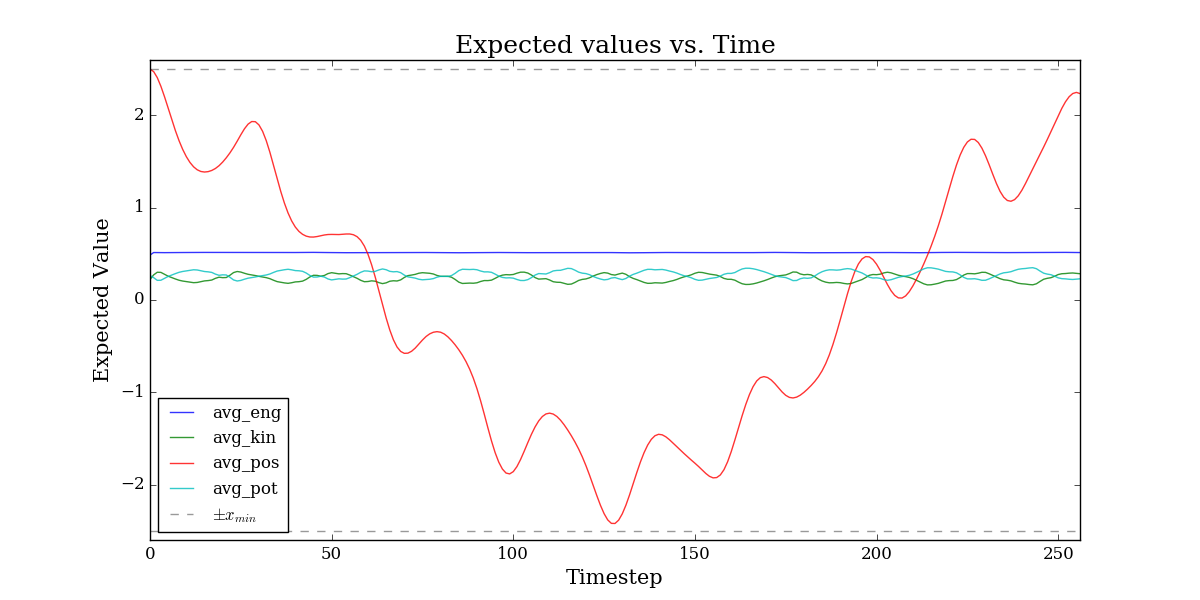
\includegraphics[width=16cm]{plots/expected.png} 
\end{center}
\end{figure}

Snapshots of the wave function at timesteps $t_s=0, 32, 64, 96, 128$:
\begin{figure}[H]
\begin{center}
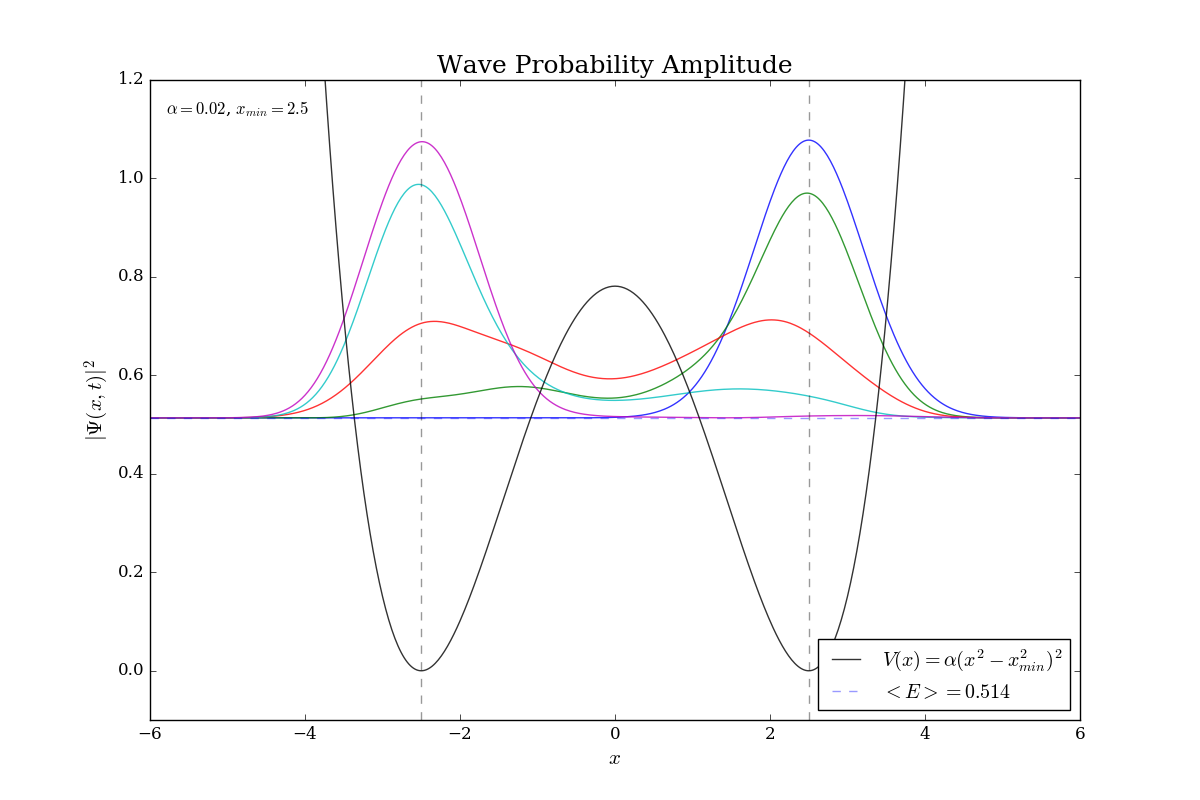
\includegraphics[width=16cm]{plots/period_sample.png}
\end{center}
\end{figure}

Since the expected position reaches a minimum at $t_s=128$, the tunneling time for this experiment is $t_s=128$. For animation, see plots/wave$\_$evolution.gif.


\bigskip
\textbf{Question 3}: Determine an approximate relation between the tunneling gap and tunneling time. \\

\textit{Solution:} \\
Let $\phi_o$ and $\phi_1$ be the two lowest energy stationary states for the solution for the double potential well, and let us define $|a\rangle$ and $|b\rangle$ as the normalized sum and difference of these two energy states:
\begin{align*}
	|a\rangle &= \frac{1}{\sqrt{2}} \left(|\phi_o\rangle + |\phi_o\rangle \right) \\
	|b\rangle &= \frac{1}{\sqrt{2}} \left(|\phi_o\rangle - |\phi_o\rangle \right)
\end{align*}
where $|b\rangle$ looks like $t_s=0$ and $|a\rangle$ looks like $t_s=128$ in the last figure, and the tunneling time is the time it takes to get from $|b\rangle$ to $|a\rangle$. 

\begin{align*}
	\langle b| e^{-iHt} |a \rangle 
	&= \langle b | \frac{1}{\sqrt{2}} \left(e^{-iE_ot} | \phi_o \rangle + e^{-iE_1t} | \phi_1 \rangle \right) \\ 
	&= \frac{1}{2} \left(e^{-iE_ot} - e^{-iE_1t} \right) \\
	||\langle b| e^{-iHt} |a \rangle || 
	&= \frac{1}{4} || 1 - e^{-i(E_1 - E_o)t} ||^2 \\
	&= \frac{1}{2} \left[1 - \cos\left(\frac{(E_1 - E_o)t}{\hbar} \right) \right]
\end{align*}
So $\frac{(E_1 - E_o)t}{\hbar} = \omega \tau$ is the time period it takes the wave function to evolve between $|b\rangle$ to $|a\rangle$, where $\tau$ is the tunneling time. Thus as the tunneling gap ($E_1 - E_o$) increases, the tunneling time decreases.


\bigskip
\textbf{Question 4}: For a free particle, show K(b,a) satisfies the Schr\"odinger Equation:
\[\frac{\hbar}{i} \frac{\partial K(b,a)}{\partial t_b} = \frac{-\hbar^2}{2m} \frac{\partial^2 K(b,a)}{\partial x_b^2} \]
where K(b,a) is:
\[K(b,a) = \sqrt{\frac{m}{2\pi i \hbar (t_b - t_a)}} e^{\frac{i m (x_b - x_a)^2}{2\hbar (t_b - t_a)}} \]

\textit{Solution}: \\
For simplification, let $\alpha = \frac{m}{2i\hbar}$.
\[K(b,a) = \sqrt{\frac{\alpha}{\pi (t_b - t_a)}} e^{\frac{-\alpha (x_b - x_a)^2}{(t_b - t_a)}} \]

The partial derivatives for K(b,a) are:
\begin{align*}
	\frac{\partial K(b,a)}{\partial t_b} 
	&= -\sqrt{\frac{\alpha}{\pi}} \left[\frac{1}{2(t_b - t_a)^{3/2}} \right] e^{\frac{-\alpha (x_b - x_a)^2}{(t_b - t_a)}} 
	+ \sqrt{\frac{\alpha}{\pi}} \left[-\frac{1}{2(t_b - t_a)^{1/2}} \right] \left[\frac{\alpha (x_b - x_a)^2}{(t_b - t_a)^2} \right] e^{\frac{-\alpha (x_b - x_a)^2}{(t_b - t_a)}} \\
	&= \sqrt{\frac{\alpha}{\pi}} \left[-\frac{1}{2(t_b - t_a)^{3/2}} + \frac{\alpha (x_b - x_a)^2}{(t_b - t_a)^{5/2}} \right] e^{\frac{-\alpha (x_b - x_a)^2}{(t_b - t_a)}} \\
	\frac{\partial K(b,a)}{\partial x_b}
	&= \sqrt{\frac{\alpha}{\pi}} \left[\frac{1}{(t_b - t_a)^{1/2}} \right] \left[\frac{-2\alpha (x_b - x_a)}{(t_b - t_a)} \right] e^{\frac{-\alpha (x_b - x_a)^2}{(t_b - t_a)}} \\
	&= -\sqrt{\frac{\alpha}{\pi}} \left[\frac{2\alpha (x_b - x_a)}{(t_b - t_a)^{3/2}} \right] e^{\frac{-\alpha (x_b - x_a)^2}{(t_b - t_a)}} \\
	\frac{\partial^2 K(b,a)}{\partial x_b^2}
	&= -\sqrt{\frac{\alpha}{\pi}} \left[\frac{2\alpha}{(t_b - t_a)^{3/2}} \right] \left[1 - \frac{2\alpha (x_b - x_a)^2}{(t_b - t_a)} \right] e^{\frac{-\alpha (x_b - x_a)^2}{(t_b - t_a)}}
\end{align*}

Plugging in $\frac{\partial K(b,a)}{\partial t_b}$ and $\frac{\partial^2 K(b,a)}{\partial x_b^2}$ to the Schr\"odinger Equation:

\begin{align*}
	\sqrt{\frac{\alpha}{\pi}} \left[-\frac{1}{2(t_b - t_a)^{3/2}} + \frac{\alpha (x_b - x_a)^2}{(t_b - t_a)^{5/2}} \right] e^{\frac{-\alpha (x_b - x_a)^2}{(t_b - t_a)}}
	&= -\sqrt{\frac{\alpha}{\pi}} \left(\frac{-i\hbar}{2m} \right) \left[\frac{2\alpha}{(t_b - t_a)^{3/2}} \right] \left[1 - \frac{2\alpha (x_b - x_a)^2}{(t_b - t_a)} \right] e^{\frac{-\alpha (x_b - x_a)^2}{(t_b - t_a)}} \\
	\left[-\frac{1}{2(t_b - t_a)^{3/2}} + \frac{\alpha (x_b - x_a)^2}{(t_b - t_a)^{5/2}} \right]
	&= \left(\frac{-i\hbar}{2m} \right) \left[\frac{2\alpha}{(t_b - t_a)^{3/2}} \right] \left[1 - \frac{2\alpha (x_b - x_a)^2}{(t_b - t_a)} \right] \\
	\left[-\frac{1}{2(t_b - t_a)} + \frac{\alpha (x_b - x_a)^2}{(t_b - t_a)^{2}} \right]
	&= \left(\frac{-i\hbar}{2m} \right) \left[\frac{2\alpha}{(t_b - t_a)} \right] \left[1 - \frac{2\alpha (x_b - x_a)^2}{(t_b - t_a)} \right] \\
	&= \underbrace{\left(\frac{2i\hbar}{m} \right) \alpha}_{\text1} \left[-\frac{1}{2(t_b - t_a)} + \frac{\alpha (x_b - x_a)^2}{(t_b - t_a)^2} \right] \\
	&= \left[-\frac{1}{2(t_b - t_a)} + \frac{\alpha (x_b - x_a)^2}{(t_b - t_a)^2} \right]
\end{align*}

Hence K(b,a) satisfies the Schr\"odinger Equation for a free particle (V(x) = 0).


\bigskip
\textbf{Question 5}: Using the equation for K show that the wavefunction 
	\[\psi(x', t') = \int^{\infty}_{-\infty} K(x', t', x, t) \psi(x,t) dx \]
satisfies the Schr\"odinger equation. \\

\textit{Solution:} \\
Using the action for a free particle $S_{cl} = \int^{t'}_{t} dt \frac{1}{2} m \dot{x}(t)^2 $, K becomes:
	\[K(x', t', x, t) = \sqrt{\frac{m}{2\pi i\hbar t}} e^{\frac{im(x' - x)^2}{2\hbar (t' - t)}} \]
as stated in the lecture notes. Let $\beta = \sqrt{\frac{m}{2\pi i\hbar t}}$, $\gamma = x' - x$, and $\alpha = t' - t$. So K can be rewritten as
	\[K = \beta e^{\frac{im}{2\alpha} \gamma^2} \]

Considering an initial condition $|\psi(x,t) \rangle$ evolved by some small amount of time $\alpha$ later, the wave function can then be described as 
	\[\psi(x, t+\alpha) = \int^{\infty}_{-\infty} K(x+\gamma, t+\alpha, x, t) \psi(x+\gamma,t) d\gamma \]

Taylor expanding the equation for $\psi$ gives us
	\[\psi(x+\gamma, t) = \psi(x,t) + \gamma \frac{d\psi(x,t)}{dx} + \frac{1}{2} \gamma^2 \frac{d^2\psi(x,t)}{dx^2} + ... \]

	\[\psi(x, t+\alpha) \approx \beta \int^{\infty}_{-\infty} d\gamma \left[\psi(x,t) +  \underbrace{\gamma \frac{d\psi(x,t)}{dx}}_{0 \Rightarrow \rm{odd \, function}} + \frac{1}{2} \gamma^2 \frac{d^2\psi(x,t)}{dx^2} \right] e^{\frac{im}{2\alpha} \gamma^2} \]

Evaluating the gaussian integral gives 
	\[\psi(x, t+\alpha) \approx \underbrace{\beta \sqrt{\frac{2\hbar \pi \alpha}{i m}}}_{1} \left[\psi + \frac{1}{2}\gamma^2 \frac{d^2\psi}{dx^2} \right]  = \left[1 - \frac{\alpha}{i\hbar} \left(\frac{\hbar^2}{2m} \frac{d^2}{dx^2} \right)\right] \psi(x,t) \]
For the limit as $\alpha \rightarrow 0$ we have
	\[\frac{d\psi(x,t)}{dt} = \frac{\psi(x,t+\alpha) - \psi(x, t)}{\alpha} \]
Hence 
	\[i\hbar \frac{d}{dt}\psi(x,t) = -\frac{\hbar^2}{2m} \psi(x,t) \]


\bigskip
\textbf{Question 6}: For a harmonic oscillator, show that the exponent of the propagator matrix has the form 
\[S_{cl} = \frac{m\omega}{2 \sin\omega T} \left[(x_a^2 + x_b^2) \cos \omega T - 2x_a x_b \right] \]

\textit{Solution}:

Solving for the action for the harmonic oscillator:

\begin{align*}
S_{cl} = \int^{t_b}_{t_a} \mathcal{L}(x, \dot{x}, t) dt = \frac{m}{2} \int^{t_b}_{t_a} (\dot{x}^2 - \omega^2 x^2) dt
\end{align*}

For the first part of the integral
\[\int^{t_b}_{t_a} \dot{x}^2 dt = \int^{t_b}_{t_a} \dot{x}\dot{x} dt = x\dot{x} \big\rvert^{t_b}_{t_a} - \int^{t_b}_{t_a} x\ddot{x} dt = x\dot{x} \big\rvert^{t_b}_{t_a} - \omega^2 \int^{t_b}_{t_a} x^2 dt \]

using $\ddot{x} = -\omega^2 x$.

\begin{align*}
	S_{cl} 
	&= \frac{m}{2} \left[x\dot{x} \big\rvert^{t_b}_{t_a} +  \omega^2 \int^{t_b}_{t_a} x^2 dt -  \omega^2 \int^{t_b}_{t_a} x^2 dt \right] = \frac{m}{2} \left[x\dot{x} \right]^{t_b}_{t_a} \\
	&= \frac{m}{2} \left[x(t_b)\dot{x}(t_b) - x(t_a)\dot{x}(t_a) \right]
\end{align*}

Now we need to plug in $x(t)$ and $\dot{x}(t)$ for $t_a = 0$ and $t_b = T$. Recall that a harmonic oscillator m\"x $= -kx$ has the general solution 
	\[x(t) = A\sin(\omega t) + B\cos(\omega t)\]
where $\omega = \sqrt{k/m}$. Applying boundary condtions $x(0) = x_a$ and $x(T) = x_b$:
	\[x(0) = B = x_a \]
	\[x(T) = A \sin(\omega T) + x_a \cos(\omega T) = x_b \]
we determine the solutions for the constants:
	\[A = \frac{x_b - x_a \cos(\omega T)}{\sin(\omega T)} \]
	\[B = x_a \]

So the particular solution for x is:
\begin{align*}
	x(t) &= \left(\frac{x_b - x_a\cos\omega T}{\sin\omega T} \right) \sin\omega T + x_a \cos\omega T \\
	\dot{x}(t) &= \left(\frac{x_b - x_a\cos\omega T}{\sin\omega T} \right) \omega \cos\omega t - x_a \omega \sin\omega t
\end{align*}

Now plugging in $t_a = 0$ and $t_b = T$ we get:
\begin{align*}
	x(0) &= x_a \\
	x(T) &= x_b \\
	\dot{x}(0) &= \left(\frac{x_b - x_a\cos\omega T}{\sin\omega T} \right) \omega \\
	\dot{x}(T) &= \left(\frac{x_b - x_a\cos\omega T}{\sin\omega T} \right) \omega \cos\omega T - x_a \omega \sin\omega T
\end{align*}

Finally, the action can be reduced to the solution above:
\begin{align*}
	S_{cl} &= \frac{m}{2} \omega \left[x_b \left(\frac{x_b - x_a\cos\omega T}{\sin\omega T} \right) \cos\omega T  -x_b x_a \sin\omega T - x_a x_b \left(\frac{x_b - x_a\cos\omega T}{\sin\omega T} \right)  \right] \\
	&= \frac{m\omega}{2\sin\omega T} \left[x_b^2 \cos\omega T - x_a x_b \cos^2\omega T - x_a x_b \sin^2\omega T - x_a x_b + x_a^2\cos\omega T \right] \\
	S_{cl} &= \frac{m\omega}{2 \sin\omega T} \left[(x_a^2 + x_b^2) \cos \omega T - 2x_a x_b \right]
\end{align*}

\end{document}